\chapter[CMS]{Content Management System}
\label{CMS}

Este capítulo tem como objetivo apresentar conceitos básicos sobre \textit{Content Management System}(CMS), que do inglês significa Sistemas Gerenciadores de Conteúdo. Nesta seção também será mostrado quais critérios serão utilizados para a escolha dos CMSs a serem avaliados futuramente no trabalho, além da revisão de literatura usada para a construção do capítulo.

\section {Revisão de literatura para o capítulo}

Na Seção \ref{Criterios_selecao} é descrito brevemente sobre os critérios de inclusão/exclusão de literatura usados neste TCC. Para este capítulo, a revisão de literatura abordou os seguintes critérios de inclusão: 

\begin{enumerate}

\item Artigos que abordem as palavras \textbf{CMS}, ou \textbf{\textit{Content Management System}}, ou \textbf{Sistemas Gerenciadores de Conteúdo}  ou quaisquer artigos que mencionem um CMS específico (\textit{Wordpress, Joomla, Drupal, Alfresco, ModX}, entre outros) no \textit{abstract} ou no título.

\item Teses, dissertações, monografias, relatórios técnicos, livros ou enciclopédias que abordem assuntos relacionados às mesmas palavras citadas no Item 1 desta seção.

\item Publicações em sites na web ou relacionadas,  porém nestes casos a publicação em sites deverá estar apoiada por outra referência de natureza citadas no Item 1 desta seção.

\end{enumerate}

Além disso, as bases de dados consultadas foram as mesmas definidas na Seção \ref{bases_de_dados}. Não foram definidas expressões de busca para este capítulo.

\section{Definições Básicas}

Um CMS é um software que mantém o controle da informação presente em uma determinada página web. Estas informações podem ser textos, fotos, músicas, vídeos, ou documentos \cite{xiang}. Ele tem como objetivo organizar, favorecer a criação, administrar, distribuir, comunicar e disponibilizar informação em um dado web site \cite{barrere}.

CMSs são uma boa solução para quem deseja organizar informações e principalmente criar e gerir conteúdos em vários contextos, dentre eles o contexto empresarial \cite{muslu}.

\subsection{CMSs e suas características}
Sistemas gerenciadores de conteúdo são softwares e todo software possui características funcionais e não funcionais que atendem aos requisitos utilizados para suas concepções.

Por este motivo, apesar deste trabalho não versar especificamente sobre requisitos de software,
a subseção seguinte faz uma breve explanação sobre os tipos de requisitos (funcionais e não funcionais) que caracterizam um CMS.


\subsubsection{Características gerais (Requisitos) de CMSs }

Para \citeonline{DePadua_2003}, requisitos são as características que delimitam os critérios de aceitação de um produto. O autor ainda acrescenta que, à medida que o processo de desenvolvimento está sendo executado, novos requisitos podem surgir, porém acrescentar características a um produto significa aumentar o custo do projeto e de sua produção. 

Segundo \citeonline{leite}, requisitos de software são o conjunto de características que expressam as necessidades dos clientes e que, ao mesmo tempo, condicionam a qualidade do software.

De acordo com \citeonline{kotonya}, requisitos de software é a caracterização de serviços que o sistema deve prover, restrições que o sistema deve possuir e conhecimentos que serão precisos para construí-lo. Conhecendo esses elementos, a atividade de análise e negociação é facilitada, pois é possível identificar os envolvidos e também o ponto de partida de um requisito. 

Os autores ainda afirmam que a Engenharia de Requisitos (ER) é a subárea da Engenharia de Software que trata do processo de definição dos requisitos de software. Esse processo é sistemático e atinge diversas atividades, tais como elicitação, análise e negociação, validação e gerência de requisitos.

%\subsubsection{Requisitos Funcionais}

\citeonline{DeBortoli} diz que requisitos funcionais definem as funções que o sistema ou componente do sistema, devem executar, ou seja, o comportamento do sistema ou de seus componentes que transforma entradas para produzir saídas.

\citeonline{cysneiros_tese} diz que os requisitos funcionais definem funções ou serviços que um software deve ser capaz de oferecer ou de executar. Estas funções ou serviços na maioria das vezes são definidas como processos que utilizam de entradas para produzir saídas.

%\subsubsection{Requisitos Não Funcionais}
De acordo com \citeonline{cysneiros97}, os requisitos não funcionais, descrevem comportamentos e restrições que o software deve possuir. 

\citeonline{DeBortoli} diz que requisitos não funcionais também são chamados de requisitos de qualidade. Esses requisitos descrevem tanto restrições no produto (desempenho, confiabilidade, interface de usuários, segurança) podendo, devido aos seus níveis de exigência, causar restrições no processo de desenvolvimento como aumento de custo e prazos de desenvolvimento.

%\subsubsection{Classificação dos Requisitos não funcionais}

Existem várias classificações para requisitos não funcionais propostas na literatura. As figuras \ref{RNF} e \ref{RNF1} são algumas delas:

\begin{figure}[h]
\centering
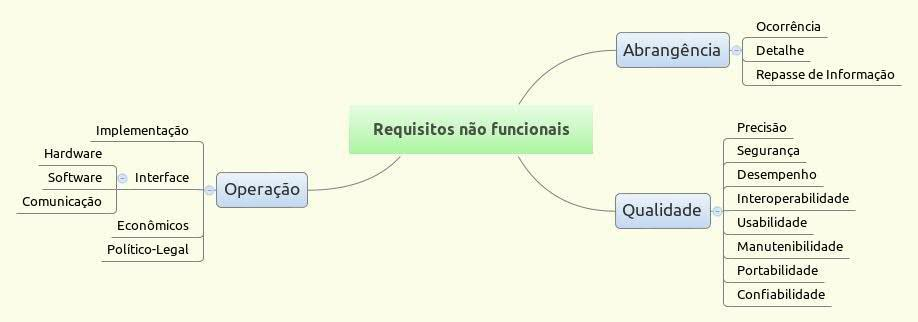
\includegraphics[keepaspectratio=true,scale=0.35]{figuras/RNF1.jpg}
\caption{Classificação de Requisitos Não Funcionais de \cite{mamani}}
\label{RNF}
\end{figure}


Já \citeonline{sommer92} apresenta uma classificação um pouco diferente. Para este autor, os requisitos não funcionais podem ser agrupados pelas seguintes Classes: Requisitos de Produto, Requisitos Externos e Requisitos de Processo.

\begin{figure}[h]
\centering
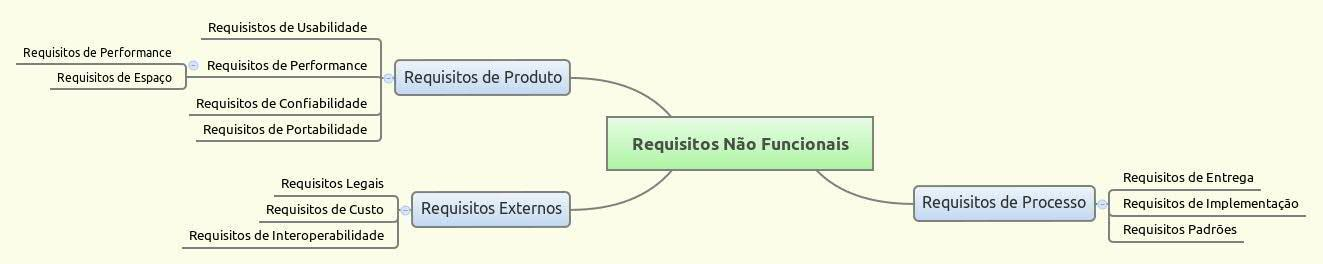
\includegraphics[keepaspectratio=true,scale=0.35]{figuras/RNF2.jpg}
\caption{Classificação de Requisitos não Funcionais por \citeonline{sommer92}.}
\label{RNF1}
\end{figure}

%\subsubsection{Requisitos Não Funcionais de Desempenho}
%\label{requisitos_nao_funcionais}
%
%Uma questão importante durante o desenvolvimento de software é saber gerenciar os requisitos de desempenho do software. Na prática, os requisitos de desempenho, muitas vezes se concentram em tempo de resposta e taxa de transferência, porém a definição de requisitos de desempenho vai muito além destes dois conceitos \cite{Nixon}. Para este autor os requisitos de desempenho merecem atenção especial, pois representam um grande desafio para sistemas de informação e para os demais sistemas de software, pois estes requisitos podem impactar de forma integral o sistema em questão. Isto é, a resposta de uma tal exigência pode alterar várias partes de um sistema. 
%Isso significa que não se pode simplesmente adicionar um módulo que melhore o desempenho do sistema como um todo, é preciso considerar o desempenho ao longo do processo de desenvolvimento.
%
%Para \citeonline{DePadua_2003}, os requisitos de desempenho são requisitos numéricos, estáticos e dinâmicos,  a que o sistema devam obedecer. São exemplos de requisitos estáticos: números de terminais suportados, números de usuários simultâneos e volume de informação que deve ser tratado.
%
%\citeonline{DePadua_2003} acrescenta dizendo que no caso de requisitos dinâmicos podem ser incluídos, por exemplo, o número esperado de transações por unidade de tempo, indicando-se condições de normalidade e de sobrecarga. Para o autor, todos os requisitos de desempenho devem ser descritos de forma quantitativa e mensurável. Isto é, um exemplo de requisito de desempenho mal definido é: “O software deverá ter resposta rápida”. O requisito aceitável seria: “90\% das vezes o tempo de resposta do software deverá ser inferior a X segundos”. Onde "X" seria um número aceitável para o usuário,
%que o deixaria satisfeito com o desempenho do sistema.
%
%\citeonline{patel}, enunciam que todos os CMSs cumprem tarefas comuns de conteúdo, como criar, editar, publicar. Um exemplo de criação é a inserção de um plugin, ou de um determinado texto no site. A edição é a alteração de um determinado conteúdo seja texto ou a troca de um determinado plugin. A publicação é o processo de gerar o conteúdo para que o mesmo possa ser mostrado no site. Mas, além desses requisitos básicos relativos a gerência de conteúdo há a preocupação com vários outros critérios que vão além da administração do conteúdo como: bom suporte ao usuário, a segurança da página, documentação entre outros. 


\subsection{Vantagens no uso de CMS para o desenvolvimento web}

O uso de CMSs no contexto de desenvolvimento web possui diversas vantagens. \citeonline{barrere}, \citeonline{costa}, \citeonline{Vantagens} e \citeonline{DosSantos} listam algumas delas:
%Para compreender o \textit{modus operandi} do STPC/DF, visitou-se as empresas Expresso São José, Sociedade de Transportes Coletivos de Brasília, Urbi Mobilidade Urbana e Viação Piracicabana. Isso permitiu a visualização da migração do antigo para o novo modelo de transporte público coletivo do Distrito Federal e a descoberta dos problemas técnicos mencionados em \ref{localizacao}, \ref{linha} e \ref{bilhetagem} e também a compreensão do monitoramento feito pelo CCO das empresas.
\begin{itemize}
\item Uso de modelos pré definidos de páginas web (os chamados templates), que garantem a consistência de exibição do site como um todo.
\item Funcionalidades podem ser incorporadas por meio de componentes pré construídos (os chamados plugins).
\item Possibilidade de construir e administrar um website sem a necessidade de conhecer linguagens de programação para web.
\item No contexto empresarial há redução de mão de obra com manutenção de sites por permitir maior desempenho no desenvolvimento.
\item Permite gerir com facilidade o conteúdo do site separadamente do design. 
\item Basta ter um browser para criação e manutenção não sendo necessários nenhum software adicional.
\end{itemize}

\subsection{Desvantagens no uso de CMS para o desenvolvimento web}

Apesar de possuir inúmeras vantagens o uso de CMS ainda apresenta algumas desvantagens. \citeonline{barrere} e \citeonline{DosSantos} listam as seguintes desvantagens, dentre outras: 
\begin{itemize}
\item Apesar de trazer consistência a página web o uso de modelos pré-definidos também impõe restrições e limitações características do modelo a ser usado.
\item A aparência do site fica limitada a quantidade de templates disponíveis para o CMS a ser usado.
\item Apesar de criar sites com facilidade e  evitar   o desenvolvimento web desde do início, para   se   utilizar   todos   os   recursos   provenientes   de   um   CMS   é   necessário   um certo   tempo   de   estudo   para   um bom   entendimento   e   aproveitamento de suas funcionalidades.
% \item Não é possível copiar localmente um projeto de página.\textcolor{red}{Rever esta referência.}
\item O backup da página é possível apenas no servidor.
\end{itemize}

\section{Uso de CMS na indústria de Software}
\label{uso_CMS}

Devido às inúmeras vantagens de utilização, o uso de CMSs na indústria de software é bastante ampla. \citeonline{barrere} e \citeonline{DosSantos} apresentam alguns exemplos de uso de CMS na indústria de software.  %na tabela \ref{Uso_CMS}:

\begin{itemize}
\item Blogs.
\item Sites para \textit{e-commerce}.
\item Sites para empresas ou instituições.
\item Comunidades virtuais.
\item Fóruns de discussão.
\item Revistas e jornais online.
\item Livros colaborativos.

\end{itemize}


%\begin{table}[!ht]
%\begin{center}
%\caption{O Uso de CMS na Indústria}
%\label{Uso_CMS}
%\begin{tabular}{|c|}\hline
% 
%\textbf{Uso de CMS na indústria de Software}\\\hline
%Blogs\\\hline
%Sites para E-commerce\\\hline
%Sites para empresas ou instituições\\\hline
%Comunidades virtuais\\\hline
%Fóruns de Discussão\\\hline
%Revistas e Jornais on-line\\\hline
%Livros colaborativos\\\hline
% 
% 
%\end{tabular}
% \end{center}
%\end{table}

\section{Critérios para a escolha de CMSs e escolha de CMSs candidatos}
\label{CMSs_candidatos}
No mercado de Software existem várias opções de CMSs disponíveis alguns muito populares e já consolidados, enquanto outros mais desconhecidos. Alguns CMSs são softwares livre enquanto outros proprietários.

O site  \citeonline{Vision}  apresenta uma visão rápida de vários produtos de CMS disponíveis no mercado. Dentre elas podem se destacar o Plone, Contao, Concrete5, Silverstripe, MODx que, embora não tão conhecidos, são citados pela \cite{Vision}.

O objetivo desta seção é justificar a escolha dos CMSs a serem alvos de estudo no trabalho. Os critérios investigados foram:

\begin{itemize}
\item \textbf{Licenciamento}: que para este trabalho foi investigado apenas o fato do CMS ser software livre ou proprietário, não se preocupando com detalhes relativos a licenças de software.
\item \textbf{Popularidade}: investigado por meio do tamanho das comunidades em redes sociais e o número de \textit{commits} nos repositórios Git Hub para os softwares livres.
\end{itemize}

\subsection{Software Livre / Software Proprietário}
\label{free_software}

A Engenharia de Software é bastante diferente se comparada com as demais engenharias. Uma diferença é que as pessoas que desenvolvem software podem publica-los para que qualquer outra pessoa use, modifique ou construa trabalhos derivados com código aberto. Estes produtos de software são os chamados softwares livre ou software \textit{open source} \cite{Yoshi}.

Softwares livres podem ser adaptados e modificados livremente para a resolução de um determinado problema \cite{aguiar2007}.

Para o software proprietário a cópia, redistribuição, ou modificação são proibidos pelo seu criador ou distribuidor e em geral apresentam alto custo restringindo a sua utilização \cite{aguiar2007}.

A Tabela \ref{tipos_CMS} apresenta 15 soluções em CMS previamente mapeadas em software livre e software proprietário. Soluções citadas pelos autores \citeonline{opensource_cms},    \citeonline{Vision}, \citeonline{marketing}, \citeonline{Vig}, \citeonline{coreMedia}, \citeonline{sherpa} e \citeonline{Carla_2009}.


% \caption{Mapeamento de Soluções de CMS em Software Livre e Software Proprietário}


\begin{longtable}{|c|c|c|}
\caption{Mapeamento de CMSs em Software Livre e Software Proprietário}  \label{tipos_CMS}\\
 	\hline
\textbf{CMS} & \textbf{Software Livre} & \textbf{Software Proprietário}\\\hline
Joomla & x & \\\hline
Drupal & x & \\\hline
WordPress & x & \\\hline
SilverStripe & x & \\\hline
Plone & x & \\\hline
Contao & x & \\\hline
Modx & x & \\\hline
Concrete5 & x & \\\hline
Pligg & x & \\\hline
Vignette &  & x\\\hline
CoreMedia &  & x\\\hline
Milenium Cross Media &  & x\\\hline
Notitia &  & x\\\hline
Vinias &  & x\\\hline
Sherpa &  & x\\\hline
\end{longtable}

Segundo \citeonline{sherpa}, valores de licenciamento de produtos de CMSs proprietários podem ser relevantes. A empresa fornecedora do Sherpa cita valores que podem chegar na ordem de grandeza de milhares de dólares por licença (10k - 75K). Assim sendo, a proposta do software livre de reduzir os custos de aquisição de licenças para o uso de produtos de software foi priorizada na escolha dos CMSs a serem estudados.
De fato, \citeonline{Karels} afirma que o uso de software livre está cada vez mais popular, pois apresenta várias vantagens, tanto do contexto de uso, quanto do contexto de desenvolvimento.  Dentre algumas vantagens \cite{Karels}:

\begin{itemize}
 \item O custo de aquisição é baixo. Embora o software proprietário possua mais opções para suporte e treinamento, o seu custo de aquisição é maior se comparado a um software livre.
 \item O apoio comunitário no processo de desenvolvimento é frequente. Dependendo da comunidade uma dúvida pode ser respondida de forma rápida, como pode demorar várias semanas para ser respondida.
 \item O projeto pode ter muitos colaboradores voluntários, porém as habilidades e a disponibilidade desses colaboradores podem variar de forma significante.
 \item Funcionalidades podem ser adicionadas com o projeto em andamento. Essa adição de funcionalidades é priorizada de acordo com as necessidades dos usuários do software livre em questão.
 
\end{itemize}

Sendo assim, as opções mapeadas como software livre foram priorizadas nas análises da próxima seção, juntamente com o critério de avaliar suas respectivas popularidades.

\subsection{Popularidade}
\label{popularidade_CMS}

O software livre vem se tornando bastante popular nos últimos anos. Essa popularidade se deve à internet, a qual permite uma distribuição rápida e em larga escala dos softwares que seguem esse modelo. Entretanto, a internet não colaborou apenas para a popularidade dos softwares livres, mas também permitiu atrair vários contribuidores bastando apenas o interesse dos mesmos \cite{salgado}. 
	
Para o conceito popularidade, serão avaliados os nove CMSs Software Livre mapeados na Seção \ref{free_software}. Para justificar este conceito foram escolhidos três parâmetros, são eles:

\begin{itemize}
\item Número de contribuições – mensurada a partir do número de \textit{commits} no repositório segundo a página das aplicações  \cite{GitHub}. Cabe ressaltar que foi preferido utilizar o número de \textit{commits} no 
repositório de contribuições de melhorias do produto, independentemente do número de pessoas cadastradas como contribuintes, na suposição de que, apesar de um número menor de contribuintes,
contribuições eram mais frequentes.
\item Número de “opiniões favoráveis” na rede social Facebook - número de pessoas na maior comunidade do CMS na rede social Facebook, segundo pesquisa realizada no site \cite{face}.
\item Número de “opiniões favoráveis” no Twitter” - número de pessoas na maior comunidade do CMS na rede social Twitter, segundo pesquisa realizada no site \cite{twitter}.
\end{itemize}

A partir das investigações feitas nos sites \cite{face}, \cite{twitter} e \cite{GitHub} foram obtidos os dados da Tabela \ref{Popularidade} \footnote{Dados atualizados até o dia 07/06/2015.}.

\clearpage

\begin{table}[!ht]
\begin{center}
\caption{Popularidade dos CMSs Mapeados }
\label{Popularidade}
\begin{tabular}{|l|l|l|l|}\hline
\textbf{CMS} & \textbf{Comunidade} & \textbf{Facebook} & \textbf{Twitter} \\\hline
Joomla &  22.064 & 159.051 & 57.064\\\hline
Drupal & 18.840 & 79.161 & 58.932\\\hline
WordPress & 29.909 & 925.419 & 1.397.303\\\hline
SilverStripe & 14.364 & 3.374 & 3.373\\\hline
Plone & 71 & 1.173 & 3.582\\\hline
Contao & 5.347 & 2.855 & 1.940\\\hline
Modx & 7.858 & 3.349 & 4.593\\\hline
Concrete5 & 13.353 & 2.268 & 5.718\\\hline
Pligg & 1.146 & 580 & 807\\\hline
\end{tabular}
\end{center}
\end{table}

As Figuras \ref{pop_001}, \ref{pop_002}, \ref{pop_003}, \ref{pop_004}, \ref{pop_005}, \ref{pop_006} mostram a visão gráfica da popularidade a partir da Tabela \ref{Popularidade}.


\begin{figure}[!ht]
\centering
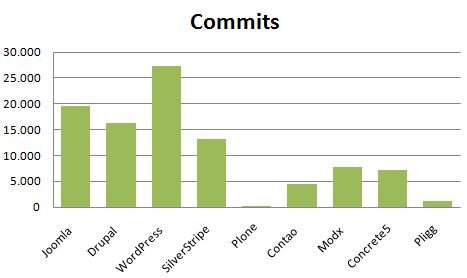
\includegraphics[keepaspectratio=true,scale = 0.8]{figuras/commits.JPG}
\caption{Popularidade pelo número de commits no git hub.}
\label{pop_001}
\end{figure}

\begin{figure}[!h]
\centering
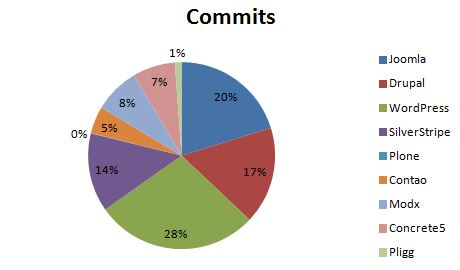
\includegraphics[keepaspectratio=true,scale = 0.9]{figuras/commits1.JPG}
\caption{Percentual de popularidade pelo número de commits no git hub.}
\label{pop_002}
\end{figure}

\clearpage
\begin{figure}[!ht]
\centering
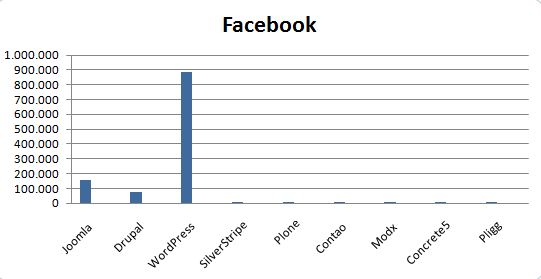
\includegraphics[keepaspectratio=true,scale = 0.9]{figuras/facebook.JPG}
\caption{Popularidade de acordo com a rede social Facebook.}
\label{pop_003}
\end{figure}


\begin{figure}[!ht]
\centering
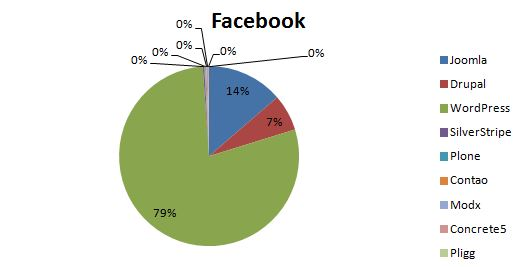
\includegraphics[keepaspectratio=true,scale = 0.9]{figuras/facebook1.JPG}
\caption{Percentual de popularidade de acordo com a rede social Facebook.}
\label{pop_004}
\end{figure}

\begin{figure}[!ht]
\centering
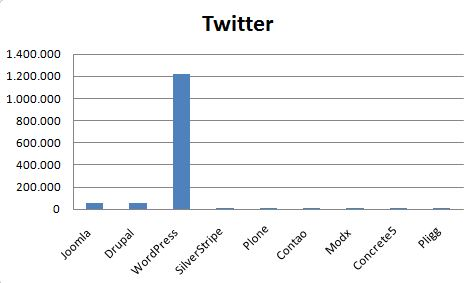
\includegraphics[keepaspectratio=true,scale = 0.9]{figuras/Twitter.JPG}
\caption{Popularidade de acordo com a rede social Twitter.}
\label{pop_005}
\end{figure}

\begin{figure}[!ht]
\centering
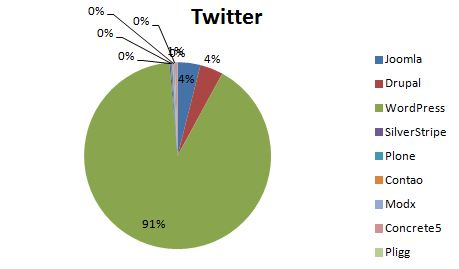
\includegraphics[keepaspectratio=true,scale = 0.8]{figuras/Twitter1.JPG}
\caption{Percentual de popularidade de acordo com a rede social Twitter.}
\label{pop_006}
\end{figure}

A partir das Figuras \ref{pop_001}, \ref{pop_002}, \ref{pop_003}, \ref{pop_004}, \ref{pop_005}, \ref{pop_006} e da Tabela \ref{Popularidade} foi constatado que os CMSs mais populares são o Wordpress, Joomla, e Drupal.

Além dos parâmetros observados outras pesquisas de sites da internet apontam os CMS mais populares.

Para a \citeonline{marketing}, o WordPress é o CMS mais usado no mundo. Ele tem licença livre, e pode ser instalado com facilidade, a empresa gosta de mencionar a sua rápida instalação de 5 minutos. Apesar de ser considerado uma plataforma feita para blogs, o WordPress é bastante mutável e pode ser usado na construção de páginas corporativas, e-commerce, jornais e demais itens mencionados na seção \ref{uso_CMS} deste trabalho. 
 
 Logo depois do WordPress aparece o Joomla como segunda ferramenta de CMS mais usada. O debate sobre qual ferramenta é a melhor já existe há muito tempo, com defensores de ambos os lados. Apesar da competição o Joomla ainda perde em quesitos como simplicidade e funcionalidades, não sendo aconselhado para pessoas iniciantes no desenvolvimento web, segundo o site \citeonline{marketing}. 

 O Drupal mesmo apresentando um crescimento no número de usuários, ainda é pequeno se comparado com WordPress ou Joomla. O sistema também é mais complexo do que seus concorrentes, não sendo indicado para usuários leigos, apenas para aqueles que já possuem alguma experiência com desenvolvimento, segundo o site \citeonline{marketing}.
% (quanto? Faz uma continha de diferença % dos dados da tabela 2 e colocar num gráfico de barras).


A \citeonline{opensource_cms}, utilizou um complemento de navegador chamado\textit{ Wappalyzer}, que tem por finalidade descobrir quais tecnologias foram usadas para a construção de tais sites. Dentre essas tecnologias que podem ser encontradas, podem-se destacar CMS, frameworks e ferramentas de análise de código. Com o auxílio desta ferramenta a OpenSource CMS, descobriu que o Wordpress, o Joomla e o Drupal são os mais utilizados na composição dos sites avaliados respectivamente, tomando como exemplo uma amostra de 1 \% de sites da internet.


Com base nas pesquisas efetuadas desta seção foram escolhidos para fazerem parte do estudo como CMSs populares: Joomla, Drupal e Wordpress.

\section{Vantagens e Desvantagens dos CMS mais populares}
\label{Cms_vantagens}

Esta seção tem como objetivo analisar algumas vantagens e desvantagens dos CMSs escolhidos Joomla, WordPress e Drupal, porém antes de mostrar as vantagens e desvantagens de tais CMSs será apresentada uma visão rápida de cada CMS. 

\begin{enumerate}
 \item \textbf{Wordpress}: É um software livre que possui licença  GPLv2\footnote{A \textit{General Public License} é uma licença projetada por Stalman para software livre possui quatro princípios básicos. Dentre esses princípios destacam-se A liberdade para executar, distribuir, desenvolver melhorias para o programa e produzir trabalhos derivados, desde que o software derivado, ou seus trabalhos derivados sejam também livres. \cite{smith}}. Ele tem como principal objetivo a criação de blogs e fornece ao seu usuário vários recursos para a criação destes blogs. Dentre esses recursos, podem ser destacados os painéis de administração, que são uma opção para definir o comportamento e a apresentação do site \cite{Reis}.
 
\item \textbf{Drupal}: Também é um software livre que possui licença GPLv2. Trabalha com alguns conceitos chaves. Como \textbf{Módulos}, que são os conjuntos de códigos que são responsáveis por prover as principais funcionalidades do Drupal; a \textbf{Taxonomia}, que é o sistema de classificação de conteúdo;  o \textbf{Tema}, que faz o gerenciamento do que é exibido no site controlando o layout, cores e aspecto gráfico \cite{Reis}.  
 
 \item \textbf{Joomla}: Distribuído sob licença GPLv2 é um CMS software livre que permite total customização do layout, tornando possível desde a simplificação de buscas até o suporte à múltiplas línguas(internacionalização)\cite{Reis}. 
 \end{enumerate}

\citeonline{costa}, \citeonline{Reis} elencam em seus trabalhos várias vantagens e desvantagens dos CMSs Joomla, Wordpress e Drupal. A relação de vantagens e desvantagens de cada CMS está na Tabela \ref{Vantagens}.

\clearpage

% \begin{table}[!ht]
 	\begin{center}
 	
 	
 	\begin{longtable}{|p{65pt}|p{140pt}|p{140pt}|}
	
	\caption{Vantagens e Desvantagens dos CMSs, segundo \cite{costa}, \cite{Reis}}
	
 	 \label{Vantagens}\\
%  	\end{longtable}

 	\hline
 	 {\raggedright \textbf{CMS}}
 	 & {\raggedright \textbf{Vantagens}}
 	 & {\raggedright \textbf{Desvantagens}}\\
 	\hline
 	 {\raggedright Joomla}
 	 & {\raggedright 
 	                  Fácil de instalar.
 	                   
 	                  Boa usabilidade.		
			   
			  Software Livre.		
			   
			  Flexibilidade e interatividade alta.
			  
			  Forte documentação.
			  
			  Comunidade bastante ativa.
			  
			  
%  	             
	    }
 	 & {\raggedright 
 	                Taxonomia Limitada.
 	                
 	                Boa parte de seus plugins e templates são pagos.
 	
 	
 	}\\
 	\hline
 	 {\raggedright Wordpress}
 	 & {\raggedright %\begin{itemize}
 	                  Fácil de instalar.
 	                  
 	                  Boa usabilidade.		
			  
			  Software Livre.		
			  
			  Flexibilidade e interatividade alta.
			  
			  Bom para a construção de blogs.
			  
			  Total conformidade com os padrões da World Wide Web Consortium. 
 	                 
 	                 
 	                 }
 	 & {\raggedright %\begin{itemize}
 	               Taxonomia Limitada.
 	               
 	               Segurança limitada.
 	               
 	               Performance Limitada.
 	               
 	               Mecanismo de busca não é preciso.
 	             
 	
 	}\\
 	\hline
 	 {\raggedright Drupal} 
 	 & {\raggedright %\begin{itemize}{
			  Boa taxonomia.
			  
			  Software Livre.
			  
			  Possui mais recursos em nível de desenvolvimento.
			  
			  Fácil configuração para interagir com outros sites e tecnologias.
			  
			  Liberdade para a alteração de um template específico.
			  
			  
			  
 	                 %\end{itemize}}
 	 
 	 }
& {\raggedright Curva de aprendizado alta.

		 Usabilidade ruim.	
		 
		 Difícil de instalar.
		 
		 Inadequado para usuários com pouca experiência no uso de CMS.

  }\\
 	\hline
 	\end{longtable}
 	
 	\end{center}
 	
A partir da Tabela \ref{Vantagens} foi constatado que os CMSs possuem vantagens em comum tais como, a facilidade de instalar e o fato de serem open source. Entretanto mesmo oferecendo várias vantagens os CMSs ainda apresentam limitações quanto a Taxonomia (Joomla e Wordpress) e curva de aprendizado e usabilidade (Drupal).


\section{Comparativos já Realizados}

\citeonline{patel} propuseram uma pesquisa que buscava avaliar três CMSs Joomla, Wordpress e Drupal com o objetivo de aferir o desempenho desses CMSs observando algumas características. A pesquisa foi composta de dois estudos de caso, em um deles as avaliações eram feitas em um servidor local. Para o servidor local, as características observadas são detalhadas na tabela \ref{patel}:


% \begin{table}[!ht]
%  	\label{patel}
 	\begin{longtable}{|p{140pt}|p{300pt}|}
 	\caption{Características avaliadas pelo experimento de \citeonline{patel}}
 	\label{patel}\\
 	\hline
 	 {\raggedright \textbf{Característica}}
 	 & {\raggedright \textbf{Descrição}}\\
 	\hline
 	 {\raggedright Tempo de carregamento da página}
 	 & {\raggedright Tempo em Milissegundos (ms).}\\
 	\hline
 	 {\raggedright Tamanho da página}
 	 & {\raggedright Tamanho total da página em (KB).}\\
 	\hline
 	 {\raggedright Total de Requisições} 
 	 & {\raggedright Número de pedidos enviados ao servidor para se carregar uma página.}\\
 	\hline
 	 {\raggedright Total de Arquivos CSS}
 	 & {\raggedright Número de arquivos CSS usados pelo CMS para fazer uma página.} \\
 	\hline
 	{\raggedright Total de arquivos JS} 
 	 & {\raggedright Número de arquivos Java Script usados pelo CMS para fazer uma página.}\\
 	\hline
 	{\raggedright PLT} 
 	 & {\raggedright Tempo em que se armazena o conteúdo na memória cache antes da página carregar.}\\
 	\hline
 	{\raggedright PS} 
 	 & {\raggedright Quantidade de dados armazenados na memória cache antes da página carregar.}\\
 	\hline
 	\end{longtable}
 	
%  \end{table}

Depois de estabelecidas as características, \citeonline{patel} estabeleceram três experimentos dentro do primeiro cenário do servidor local:

\begin{itemize}
\item 1ª Experimento - Página comum sem plugins.
\item 2ª Experimento - Plugin de calendário e informação textual.
\item 3ª Experimento - Calendário, informação textual, imagem, plugin de relógio.
\end{itemize}

Após os dados levantados, \citeonline{patel}, obtiveram o ranking mostrado na Tabela \ref{tabela_patelc} e nas Figuras \ref{Rank1}, \ref{Rank2}, \ref{Rank3}.

\clearpage 

 \begin{table}[ht]
\begin{center}
\caption{Ranking gerado a partir do experimento de \citeonline{patel}.}
 \label{tabela_patelc}
\begin{tabular}{|l|l|l|l|}\hline
CMS/ Experimento & \textbf{Wordpress} & \textbf{Joomla} & \textbf{Drupal}\\\hline
\textbf{1ª Experimento} & 2ª & 3ª & 1ª\\\hline
\textbf{2ª Experimento} & 3ª & 2ª & 1ª\\\hline
\textbf{3ª Experimento} & 3ª & 1ª & 2ª\\\hline
 \end{tabular}
 \end{center}
  \end{table}
  
\begin{figure}[!ht]
\centering
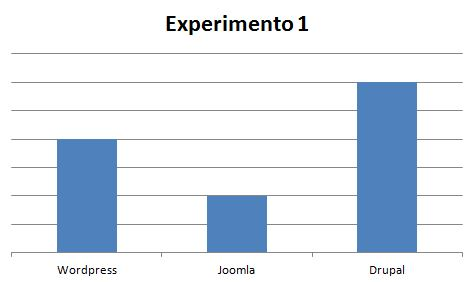
\includegraphics[keepaspectratio=true,scale=0.7]{figuras/exp001.JPG}
\caption{Ranking de melhor desempenho no experimento 1}
\label{Rank1}
\end{figure}  

\begin{figure}[!ht]
\centering
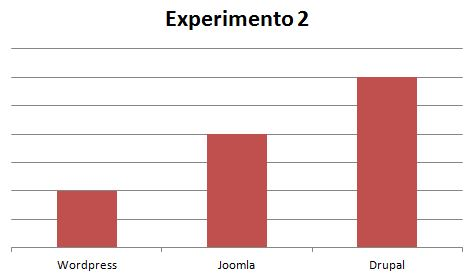
\includegraphics[keepaspectratio=true,scale=0.7]{figuras/exp002.JPG}
\caption{Ranking de melhor desempenho no experimento 2}
\label{Rank2}
\end{figure} 

\begin{figure}[!htb]
\centering
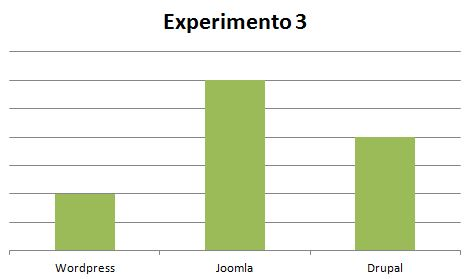
\includegraphics[keepaspectratio=true,scale=0.65]{figuras/exp003.JPG}
\caption{Ranking de melhor desempenho no experimento 3}
\label{Rank3}
\end{figure} 

\clearpage

As Figuras \ref{Rank1}, \ref{Rank2}, \ref{Rank3} e a Tabela \ref{tabela_patelc} demonstram que \citeonline{patel} obtiveram a conclusão que para um servidor local e os experimentos propostos o CMS Drupal obteve o melhor desempenho e o WordPress o pior.



%Levando em consideração os experimentos feitos por \citeonline{patel} a grande diferença deste TCC consiste em haver um catálogo de métricas que será desenvolvido com base na ISO-IEC 9126 e estruturado segundo o método GQM apresentado na seção \ref{GQM}. O que não foi explicitado pelos autores nos seus estudos.

%Assim sendo a contribuição deste estudo consistiu em respaldar as medições  escolhidas a partir de características de qualidade referenciadas pela norma ISO 9126 para, a partir delas, estabelecer o conjunto de medições a serem usadas no contexto da característica de desempenho.
%Além disso, as medições serão submetidas a avaliação de especialistas(como previsto em TCC 2), para averiguar suas relevâncias e facilidades(ou dificuldades) de execução. Com este procedimento pretende-se obter um framework de medições mais útil e alinhado aos reais interesses dos responsáveis pela
%escolha de um determinado CMS para o desenvolvimento de um determinado software em ambiente WEB e sob o aspecto de desempenho. Desta forma o estudo poderia ser repetido de forma semelhante para outras características não funcionais de interesse futuramente, como: manutenibilidade, confiabilidade, etc.

Conforme visto, características carecem de definições mais objetivas para poderem ser considerados como bem definidos. Uma forma de objetivamente quantificar grandezas consiste em utilizar a teoria de métricas de software. A \citeonline{iso_25000} propõe um conjunto de métricas para avaliar grandezas ligadas ao conceito de qualidade em software o que, por sua vez, será o foco de estudo dos próximos capítulos para o objetivo de definir um método baseado em características de CMS. Um método  que poderá ser utilizado como insumo para a escolha de um determinado CMS em uma organização.

\chapter[Qualidade de Software]{Qualidade de Software}
\label{Qualidade_de_Software}

%Qualidade de Software é um conceito amplo que possui vários focos pelos quais ela pode ser avaliada,por exemplo, a qualidade do produto é a qualidade que poder ser obtida por quem usa o produto de software \cite{iso_25000}.
%
%A qualidade de software varia e depende dos princípios que serão aplicados. Algumas das medidas mais comuns sobre qualidade de software avaliam, por exemplo se o software não apresenta erros, se ele funciona como previsto ou se o software produz resultados precisos. \apud{Jones}{Hamid}.

\citeonline{Hamid} dizem que medir a qualidade do software na indústria não é uma tarefa fácil e a maioria das empresas não costumam implementar este conceito. Existem várias razões para que a qualidade não seja medida, dentre alguns dos motivos mais comuns estão os gestores que não sabem como medir, dificuldades para criar a infraestrutura necessária para a medição e o medo do resultado  \apud{Kan}{Hamid}.

Durante muito tempo no contexto de desenvolvimento de software no Brasil, o uso da \citeonline{Nbr_9126}, apesar de não atingir a maioria das empresas foi maior dentre todas as normas utilizadas por empresas de software que desejassem alcançar a qualidade de seus produtos \cite{Marinho}. Os autores afirmam que 5,7 \% de 343 organizações pesquisadas utilizam a \citeonline{Nbr_9126} como padrão para se alcançar a qualidade de software.

Porém a norma ISO 9126 foi substituída pela série de normas 25000, também chamadas de \textit{Software Quality Requirements and Evaluation} (SQuaRE). As Normas SQUARE trazem conceitos comuns com a antiga ISO 9126, além de novos conceitos apresentados a partir da Seção \ref{25000} \cite{iso_25010}.

\section {Revisão de literatura para o capítulo}

Para este capítulo a revisão de literatura abordou os seguintes critérios de inclusão:

\begin{enumerate}

\item  Artigos que abordassem as palavras \textbf{Qualidade de Software}, ou \textbf{\textit{Software Quality}}, ou \textbf{SQuaRE}, ou relacionadas no seu \textit{abstract} ou no seu título.

\item Teses, dissertações, monografias, relatórios técnicos, livros ou enciclopédias que abordassem assuntos relacionados as mesmas palavras citadas no item 1 desta seção.

\item Publicações em sites na web ou relacionadas,  porém nestes casos a publicação em sites foi apoiada por outra referência de natureza citadas no Tópico 1 desta seção.

\end{enumerate}

As bases de dados consultadas foram as mesmas definidas na Seção \ref{bases_de_dados}.


\section{As Normas SQuaRE}
\label{25000}

A maior motivação para a criação das Normas SQuaRE foi a necessidade de se construir um conjunto harmônico de documentos, visto que faltava clareza na utilização das normas de qualidade de produto. A SQuaRE visa obter uma série logicamente organizada e unificada com abrangência de dois processos principais: especificação de requisitos de qualidade e avaliação da qualidade de software, apoiados por um processo de medição \cite{iso_25000}.

De acordo com a \citeonline{iso_25000}, os principais benefícios da série SQuaRE em Relação aos modelos anteriores são:


\begin{itemize}

\item Coordenar a orientação sobre a mensuração da qualidade dos produtos de software e avaliação da qualidade de software. 

\item Oferecer uma orientação para a especificação de requisitos de qualidade do produto de software.

\item Harmonizar com a norma ISO/IEC 15939- Qualidade do processo de software \citeonline{iso_15939}, sob a forma de produto de Software de Qualidade de medição de referência.
 
\end{itemize}

\section{Organização das normas Square}

A Figura \ref{Org_SQuaRE} a seguir mostra a organização das normas SquaRE:

\begin{figure}[!ht]
\centering
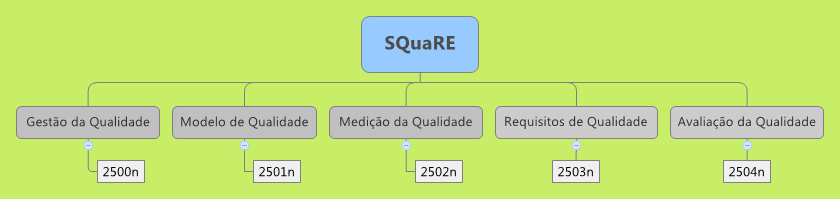
\includegraphics[keepaspectratio=true,scale=0.5]{figuras/SQuaRE.png}
\caption{Organização da série SQuaRE \cite{iso_25000}}
\label{Org_SQuaRE}
\end{figure} 

De acordo com a Figura \ref{Org_SQuaRE} as normas SQuaRE possuem como extensão:

\begin{enumerate}
\item \textbf{ISO/IEC 2500n – Divisão Gestão da Qualidade}: essa divisão determina os modelos, termos e definições a respeito das demais normas da série Square.

\item \textbf{ISO/IEC 2501n – Divisão Modelo de Qualidade}: essa divisão apresenta um modelo de qualidade detalhado, incluindo características de qualidade do produto e qualidade em uso. Além disso, as características de qualidade de produto são quebradas em subcaracterísticas. Essa divisão também oferece orientação a respeito do uso do modelo de qualidade.

\item \textbf{ISO/IEC 2502n – Divisão Medição da Qualidade}: essa divisão apresenta um modelo de referência para a medição de produtos de software, definições matemáticas das medidas de qualidade e orientações praticas para a sua aplicação. As medidas apresentadas aplicam-se ao contexto de qualidade em uso e qualidade do produto.

\item \textbf{ISO/IEC 2503n – Divisão Requisitos de Qualidade}: essa divisão especifica o que são requisitos de qualidade. Estes requisitos podem ser usados no processo de elicitação de um produto de software a ser desenvolvido ou como entrada para um processo de avaliação.

\item \textbf{ISO/IEC 2504n – Divisão Avaliação da Qualidade}: essa divisão fornece requisitos, recomendações e orientações para a avaliação de produtos de software quando realizado por avaliadores, adquirentes ou desenvolvedores.

\end{enumerate}

\section{Qualidade de Software segundo a SQuaRE}

Segundo a \citeonline{iso_25010}, a qualidade de um sistema é o grau em que o sistema satisfaz as necessidades explícitas e implícitas de seus usuários e, dessa forma, agrega valor. Estas necessidades explícitas e implícitas são representadas na série SquaRE de normas de modelos de qualidade que categorizam a qualidade do produto em características que, em alguns casos, são ainda subdivididas em subcaracterísticas.						

Esta decomposição hierárquica fornece uma análise conveniente de qualidade do produto, pois as características de qualidade definidas abrangem todos os aspectos de qualidade que são relevantes para a maioria dos produtos de software. Dessa forma, eles podem ser usados como uma lista de verificação para garantir a abrangência da qualidade \cite{iso_25010}.

Para se chegar às medidas de características de qualidade ou subcaracterísticas, é necessário identificar um conjunto de propriedades que juntos atendem a característica ou subcaracterística. Após a identificação das propriedades é necessário identificar medidas para cada uma das propriedades encontradas. A partir da identificação das medidas das propriedades pode-se chegar a medidas derivadas que sirvam de insumos para medição de características e de subcaracterísticas \cite{iso_25010}.

A \citeonline{iso_25010}  classifica a qualidade do software em características que estão subdivididas em subcaracterísticas de qualidade, conforme ilustra a Figura \ref{QualProdSoft} apresentada a seguir: 

\begin{figure}[!ht]
\centering
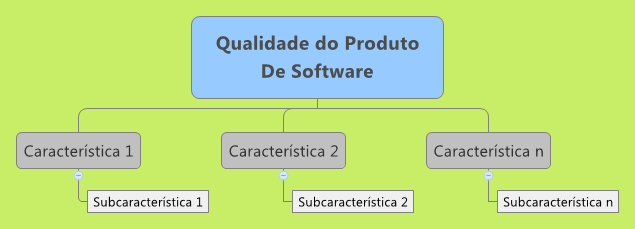
\includegraphics[keepaspectratio=true,scale=0.6]{figuras/qualidade.png}
\caption{Estrutura do modelo de qualidade da SQuaRE \cite{iso_25010}}
\label{QualProdSoft}
\end{figure}

Além disso, o modelo de qualidade  é dividido em modelo de qualidade de uso e modelo de qualidade do produto \cite{iso_25000}.

%
%\textcolor{red}{Ver uma nova palavra para substituir “atributo”}.



\subsection{O Modelo de Qualidade em Uso da Square}

A qualidade em uso define cinco características relacionadas à evolução da interação com um sistema. Essas características, segundo a \citeonline{iso_25010} são:

\begin{enumerate}
 \item \textbf{Efetividade}: é a característica que diz respeito a capacidade que o software possui de atender a metas específicas sob condições particulares de uso levando em consideração a exatidão e a integridade.
 
\item \textbf{Eficiência}: é a característica que diz respeito a capacidade que o software possui de apresentar recursos que foram gastos ao atingir metas específicas sob condições particulares de uso levando em consideração a exatidão e a integridade.

\item \textbf{Satisfação}: é a característica que diz respeito a capacidade que o software possui de agradar seus clientes em um contexto de uso específico.


\item \textbf{Inexistência de risco}: é a característica que diz respeito a capacidade que o software possui de minimizar riscos econômicos, humanos, para a vida humana e ambientais em um contexto de uso específico.

\item \textbf{Cobertura de Contexto em Uso}:  é a característica que diz respeito a capacidade que o software tem de possuir eficácia, eficiência inexistência de riscos e satisfação do cliente diante de um contexto de uso específico.


\end{enumerate}


Essas características ainda podem ser quebradas em outras subcaracterísticas e essas podem ser mensuradas por meio de métricas de qualidade em uso \citeonline{iso_25010}, conforme mostra a Figura \ref{Qualidade_uso}.

\begin{figure}[!ht]
\centering
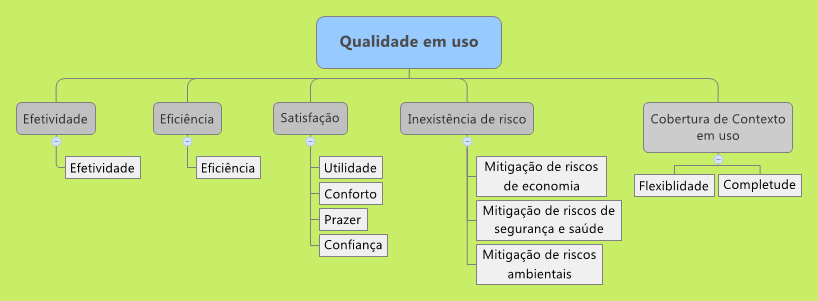
\includegraphics[keepaspectratio=true,scale=0.6]{figuras/QualidadeUso.png}
\caption{Qualidade em Uso segundo a SQuaRE \cite{iso_25010}}
\label{Qualidade_uso}
\end{figure}

\subsection{O Modelo de Qualidade do Produto segundo a norma Square}

O modelo de qualidade do produto caracteriza um sistema ou software em oito características. Essas características segundo a  \citeonline{iso_25010} são:


\begin{itemize}

\item \textbf{Adequação Funcional}: característica que diz que um produto ou sistema deve fornecer funções que correspondam às necessidades explícitas e implícitas, quando usado sob condições especificadas.


\item \textbf{Eficiência de Desempenho}: característica que estabelece o desempenho de um determinado sistema em relação à quantidade dos recursos utilizados sob condições estabelecidas.

\item \textbf{Compatibilidade}: característica que estabelece que um produto, sistema ou componente deve trocar informações e / ou realizar suas funções necessárias, ao compartilhar o mesmo ambiente de hardware ou software.


\item \textbf{Usabilidade}: característica que estabelece que um produto ou sistema deve ser usado por um usuário específico para o alcance de metas específicas com eficácia, eficiência e satisfação em um contexto de uso determinado.

\item \textbf{Confiabilidade}: característica que diz que um sistema, produto ou componente executa funções específicas sob condições determinadas em um dado período de tempo.

\item \textbf{Segurança}: característica que diz que um sistema ou produto protege as informações e dados, de modo que as pessoas, outros produtos ou sistemas possuam o grau de acesso de dados apropriado para os seus tipos e níveis de autorização.

\item \textbf{Manutenibilidade}: característica que diz que um sistema possui a capacidade de ser modificado com determinado grau de eficácia e eficiência por um conjunto de mantenedores.

\item \textbf{Portabilidade}: característica que diz que um sistema, produto ou componente pode ser transferido a partir de um hardware, software ou outro ambiente operacional com determinado grau de eficácia e eficiência.


\end{itemize}

Essas características ainda podem ser quebradas em outras subcaracterísticas e essas podem ser mensuradas por meio de métricas de qualidade do produto \citeonline{iso_25010}, conforme mostra a Figura \ref{Qualidade_Produto}.

\begin{landscape}
\begin{figure}[h]
\centering
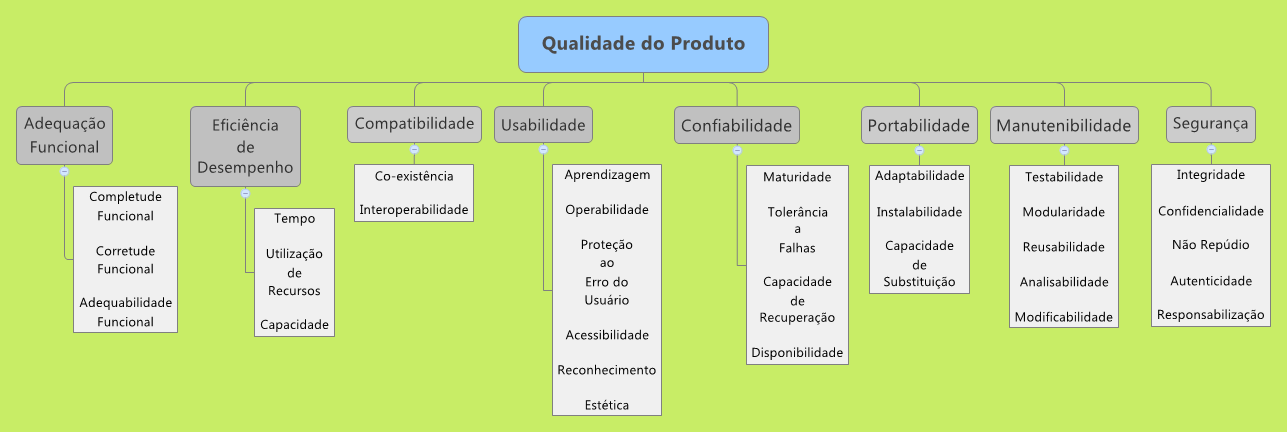
\includegraphics[keepaspectratio=true,scale=0.55]{figuras/QualidadeProduto.png}
\caption{Qualidade do Produto segundo a SQuaRE \cite{iso_25010}  }
\label{Qualidade_Produto}
\end{figure}
\end{landscape}

\subsection{Comparação entre a SquaRE e a ISO / IEC 9126 }

A SquaRE revisa a \citeonline{9126}, e mantem alguns conceitos de qualidade de software enquanto acrescenta outras características com algumas alterações.
 
 
A tabela \ref{Square_ISO} mostra um comparativo entre o que existe na SQuaRE e o que existia na antiga ISO 9126 de forma equivalente.  

\begin{longtable}{|p{12pt}|p{103pt}|p{135pt}|p{175pt}|}
 	\caption{SQuaRE X ISO 9126 \cite{iso_25010}}
 	 \label{Square_ISO}\\
 	\hline
 	 {\raggedright \textbf{\#}}
 	 & {\raggedright \textbf{Tem na Square}}
 	 & {\raggedright \textbf{Como era na ISO 9126}}
 	 & {\raggedright \textbf{Notas de Mudança}}\\
 	\hline
 	 {\raggedright 1}
 	 & {\raggedright Qualidade em uso }
 	 & {\raggedright Qualidade em uso}
 	 & {\raggedright Manteve o nome, porém uma subcaracteristica foi acrescentada e houve mudanças nas subcaracterísticas que já existiam.}\\
 	\hline
 	 {\raggedright 1.1}
 	 & {\raggedright Efetividade}
 	 & {\raggedright Efetividade}
 	 & {\raggedright Não houve alterações.}\\
 	\hline
 	 {\raggedright 1.2} 
 	 & {\raggedright Eficiência}
 	 & {\raggedright Produtividade}
	 & {\raggedright Nome alinhado com eficiência em ISO / IEC 25062 e ISO 9241-11.}\\
 	\hline
 	 {\raggedright 1.3}
 	 & {\raggedright Inexistência de Risco}
 	 & {\raggedright Segurança}
 	 & {\raggedright O conceito de segurança em nível de uso foi mudado e passou a abranger a capacidade que o sistema tem de lidar com riscos. Além disso foram acrescentadas subcaracterísticas.} \\
 	\hline
 	{\raggedright 1.4}
 	 & {\raggedright Cobertura do Contexto em Uso}
 	 & {\raggedright Não existia}
 	 & {\raggedright Foram adicionadas na qualidade em uso como subcaracterísticas completude e flexibilidade.} \\
 	\hline
 	{\raggedright 1.5}
 	 & {\raggedright Satisfação}
 	 & {\raggedright Satisfação}
 	 & {\raggedright Não existiam subcaracterísticas.} \\
 	\hline
 	{\raggedright 2}
 	 & {\raggedright Qualidade do Produto}
 	 & {\raggedright Qualidade externa/ Qualidade interna }
 	 & {\raggedright Ambos os conceitos de qualidade interna e externa foram extintos e combinados em um único conceito chamado de qualidade do produto.} \\
 	\hline
 	{\raggedright 2.1}
 	 & {\raggedright Adequação Funcional}
 	 & {\raggedright Funcionalidade}
 	 & {\raggedright Além de ter sido renomeada para adequação funcional para evitar confusão com outros sentidos de funcionalidade as subcaracteríticas que existiam na ISO 9126 foram substituídas por completude, corretude e adequação funcional.} \\
 	\hline
 	{\raggedright 2.2}
 	 & {\raggedright Eficiência de Desempenho}
 	 & {\raggedright Eficiencia}
 	 & {\raggedright Foi renomeado para evitar conflito com a definição de eficiência na ISO/IEC 25062, além disso, foi adicionada uma nova subcaracterística chamada capacidade.} \\
 	\hline
 	{\raggedright 2.3}
 	 & {\raggedright Compatibilidade}
 	 & {\raggedright Não existia}
 	 & {\raggedright  Nova característica. Inclui como subcaracterísticas interoperabilidade e co-existência.} \\
 	\hline
 	{\raggedright 2.4}
 	 & {\raggedright Usabilidade}
 	 & {\raggedright Usabilidade.}
 	 & {\raggedright Algumas subcaracterísticas foram renomeadas. A subcaracterística Acessibilidade foi acrescentada.} \\
 	\hline
 	{\raggedright 2.5}
 	 & {\raggedright Confiabilidade}
 	 & {\raggedright Confiabilidade}
 	 & {\raggedright Foi acrescentada a subcaracterística de disponibilidade.} \\
 	\hline
 	{\raggedright 2.6}
 	 	 & {\raggedright Segurança}
 	 	 & {\raggedright Subcaracterística de Funcionalidade}
 	 	 & {\raggedright Foi adicionada como uma característica, em vez de uma subcaracterística de funcionalidade, com subcaracterísticas confidencialidade, integridade, não-repúdio, prestação de contas e autenticidade.} \\
 	 	\hline
 	 {\raggedright 2.7}
 	  	 & {\raggedright Manutenibilidade}
 	  	 & {\raggedright Manutenibilidade}
 	  	 & {\raggedright Foram adicionadas duas novas subcaracterísticas a reusabilidade e a modularidade.} \\
 	  	\hline
 	  	{\raggedright 2.8}
 	  	 	 & {\raggedright Portabilidade}
 	  	 	 & {\raggedright Portabilidade}
 	  	 	 & {\raggedright A subcaracterística co-existência foi movida para a característica de compatibilidade.} \\
 	  	 	\hline
 	\end{longtable}
 
%\textcolor{red}{Colocar motivação para o próximo capítulo}

Os modelos de qualidade de software utilizam-se de medições. A medição é vital para a compreensão, controle e melhoria na engenharia \cite{tarhan}.  O capítulo \ref{metrics} define conceitos básicos de medição, medidas de software, e métodos usados para a definição de métricas.




\chapter[Métricas de Software]{Métricas de Software}
\label{metrics}

Medição é o processo no qual são atribuídos números e símbolos as características dos itens do mundo real de modo que seja possível descrever com clareza esses atributos \cite[p.~5]{Fenton}.

O resultado numérico é chamado de medida e este resultado pode ser aplicado tanto ao processo de desenvolvimento de software, quanto a um produto de software \cite{sollingen}. Além disso, uma medida pode ser considerada como uma indicação quantitativa da extensão, dimensão, tamanho ou capacidade de um determinado atributo de um processo ou produto \cite[p.~81]{pressman}.

Este capítulo tem como objetivo apresentar uma breve noção sobre tipos de métricas de software e métodos para a definição de métricas.

\section {Revisão de literatura para o capítulo}

A Seção \ref{Criterios_selecao} apresenta critérios de inclusão e exclusão de literatura usados neste TCC. A revisão de literatura deste capítulo considerou os seguintes critérios de inclusão:

\begin{enumerate}

\item Artigos que abordem as palavras \textbf{Métricas de Software}, ou \textbf{\textit{GQM}}, ou \textbf{\textit{PSM}} ou \textbf{\textit{Software Metrics}} no seu \textit{abstract} ou no seu título.

\item Teses, dissertações, monografias, relatórios técnicos, livros ou enciclopédias que abordem assuntos relacionados as mesmas palavras citadas no item 1 desta seção.

\item Publicações em sites na web ou relacionadas,  porém nestes casos a publicação em sites deverá estar apoiada por outra referência de natureza citadas no tópico 1 desta seção.

\end{enumerate}

As bases de dados consultadas foram as mesmas definidas na Seção \ref{bases_de_dados}. Não foram definidas strings de pesquisa para este capítulo.


%A medição dos atributos das entidades que compõe o software é o processo  de definir, e continuamente coletar e analisar os dados com o objetivo de compreender ou controlar o processo de desenvolvimento de software e seus produtos, para fornecer informações relevantes para a melhoria do processo de desenvolvimento \cite{sollingen}.

\section{Tipos de Métricas de Software}

Para um processo de desenvolvimento de software ou um produto ser medido é necessário o uso de métricas. Em um processo de medição podem ser usadas várias métricas ao mesmo tempo e essas mesmas métricas podem se repetir várias vezes \cite{sollingen}. Durante a medição de um produto de software, as métricas podem ser mapeadas de diversas formas \cite[pp~45-46]{Fenton}. 

Várias classificações de métricas de software podem ser encontradas na literatura, algumas delas são descritas por  \citeonline[pp.~37-42, 60, 74-83]{Fenton}, \citeonline{moller}, \citeonline[p~.9]{park} e apresentados na Tabela \ref{tipos_metricas1}:

% \begin{table}
 	\begin{longtable}{|p{70pt}|p{220pt}|p{135pt}|}
 	\caption{Tipos de métricas de Software.} \label{tipos_metricas1}\\
 	\hline
 	 {\raggedright \textbf{Classificação}}
 	 & {\raggedright \textbf{Finalidade}}
 	 & {\raggedright \textbf{Exemplo}}\\
 	\hline
 	 {\raggedright Métricas de Produto}
 	 & {\raggedright Medir atributos de produtos, documentos e artefatos oriundos do processo de desenvolvimento de software.}
 	 & {\raggedright Tamanho do produto de software.}\\
 	\hline
 	 {\raggedright Métricas de Processo}
 	 & {\raggedright Medir atividades do processo de desenvolvimento de software.}
 	 & {\raggedright Densidade de defeitos de testes.}\\
 	\hline
 	 {\raggedright Métricas de Recurso} 
 	 & {\raggedright Medir atributos que são usados durante a execução do processo de desenvolvimento de software.}
& {\raggedright Tamanho da equipe.}\\
 	\hline
 	 {\raggedright Métricas Objetivas}
 	 & {\raggedright Pode ser quantificada por meio de expressões numéricas ou gráficos.}
 	 & {\raggedright Tempo de execução.} \\
 	\hline
 	{\raggedright Métricas Subjetivas}
 	 & {\raggedright Necessitam de avaliação pessoal.}
 	 & {\raggedright Nível de satisfação do cliente,  definida em classes como: baixa, média e alta.} \\
 	\hline
 	{\raggedright Métricas Diretas}
 	 & {\raggedright Mede interações em apenas uma única dimensão.}
 	 & {\raggedright Número de funcionalidades, Esforço.} \\
 	\hline
 	{\raggedright Métricas Indiretas}
 	 & {\raggedright Mede interações entre mais de uma  dimensão.}
 	 & {\raggedright Produtividade.} \\
 	\hline
 	
 	\end{longtable}

Além das classificações sobre tipos de medições, outro conceito importante é o relativo às escalas de medição.
 	
As escalas de medição definem várias maneiras em que uma métrica pode ser mapeada por meio de relações numéricas e empíricas. O uso de escalas de medição ajuda a entender o comportamento de entidades e definir valores para seus atributos \cite[pp~45-46]{Fenton}.A Tabela \ref{tipos_metricas2} apresenta as escalas de métricas mais usadas na Engenharia de Software.

%\pagebreak
\clearpage
	\begin{longtable}{|p{70pt}|p{220pt}|p{135pt}|}

 	\caption {Tipos de escalas de métricas de Software Fonte: \cite[p. 9]{park}; \cite [pp. ~45-53]{Fenton}} \label{tipos_metricas2}\\
 	\hline
 	 {\raggedright \textbf{Tipo}}
 	 & {\raggedright \textbf{Descrição}}
 	 & {\raggedright \textbf{Exemplos}}\\
 	\hline
 	 {\raggedright Nominal}
 	 & {\raggedright Um nome ou rótulo é atribuído como classe de valor do atributo, não existindo noção de ordem entre elas. Qualquer sistema simbólico ou representação é uma medida aceitável, mas não existe noção de magnitude associada.}
 	 & {\raggedright Cor dos olhos de pessoas, classes de defeitos, nomes de linguagens, classes de custos (custos diretos, custos indiretos), etc.}\\
 	\hline
 	 {\raggedright Ordinal}
 	 & {\raggedright Semelhante à escala anterior, mas acrescenta a noção de ordem entre os tipos estabelecidos. Números, se utilizados, significam apenas classificações e não é possível efetuar operações matemáticas com eles.}
 	 & {\raggedright Os níveis de maturidade do CMM 
 	 (níveis de 1 a 5);
 	 Complexidade de uma função de um sistema (baixa, média, alta).
 	 }\\
 	\hline
 	 {\raggedright Intervalar} 
 	 & {\raggedright Preserva a importância da ordem dos resultados da escala ordinal, e ainda possui informações sobre o tamanho dos intervalos que separam seus pontos. Permite realizar adições e subtrações, mas não permite multiplicações e divisões.}
& {\raggedright Temperatura, intervalos de: datas, horários, etc.}\\
 	\hline
 	 {\raggedright Racional}
 	 & {\raggedright Preserva a ordem, o tamanho dos intervalos entre entidades, mas apresenta também as razões entre elas.
 	 Incorpora o elemento zero absoluto (representando a total falta do atributo). Todas as funções aritméticas podem ser utilizadas aplicadas em cada intervalo do mapeamento, gerando resultados significativos.
 	 }
 	 & {\raggedright Tamanho, peso, altura, tempo entre falhas, valores de custos, prazos, esforços, etc.} \\
 	\hline
 	{\raggedright Absoluta}
 	 & {\raggedright Consiste em um tipo especial de escala racional, na qual somente são admissíveis multiplicadores unitários, isto é, a medição é realizada por meio da contagem do número (quantidade) de elementos de uma determinada entidade.}
 	 & {\raggedright Número de defeitos encontrados no software, número de pessoas trabalhando em uma equipe, número de ocorrências de um determinado tipo, etc.} \\
 	\hline
 	
 	\end{longtable}
 
 \clearpage
 Na Engenharia de Software existem abordagens que auxiliam na definição das métricas, tanto de produtos, quanto de processos de software e recursos. Dois exemplos de métodos bem conhecidos são o \textit{Goal Question Metric} (GQM) e o \textit{Practical Software Measurement}(PSM).

\section{GQM}
\label{GQM}

O método \textit{Goal, Question, Metric} (GQM)  é uma abordagem utilizada para a medição composta por quatro fases\cite{sollingen}, conforme mostra a figura \ref{Fases_GQM}.

\begin{figure}[h]
\centering
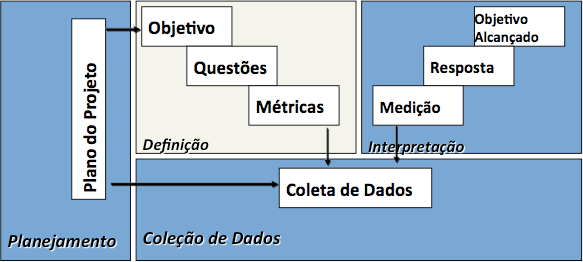
\includegraphics[keepaspectratio=true,scale=0.7]{figuras/GQM_fases.png}
\caption{Fases do GQM \cite{sollingen}}
\label{Fases_GQM}
\end{figure}

A Figura \ref{Fases_GQM} apresenta quatro fases, sendo elas:  planejamento, definição, coleta de dados e interpretação. Cada uma delas é explicada a seguir.

\begin{enumerate}
\item \textbf{Fase do Planejamento}: nesta fase o planejamento da definição das medições é feito, com atividades características como: escolher o(s) objetos(s) a serem mensurados, com suas características para que sejam avaliadas por meio de medições. Além disso, a equipe que trabalhará no projeto de definições será formada, assim como todas as etapas do trabalho serão configuradas \cite{card}. 

\item \textbf{Fase de Definição}: nesta fase a estratégia de medição é estabelecida. São definidos os objetivos, as questões, as métricas e as hipóteses e essas definições são documentadas \cite{card}.

\item \textbf{Fase de Coleta de Dados}: nesta fase a coleta de dados ocorre resultando em um levantamento de dados \cite{card}.

\item \textbf{Fase da Interpretação}: nesta fase os dados são processados de acordo com as métricas definidas para a medição dos resultados, para que as respostas das questões sejam encontradas e para que os objetivos possam ser avaliados \cite{card}.

\end{enumerate}

 
Para \citeonline{Basili}, o GQM pode ser dividido em três níveis principais, conforme ilustra a Figura \ref{Niveis_GQM}:

\begin{figure}[h]
\centering
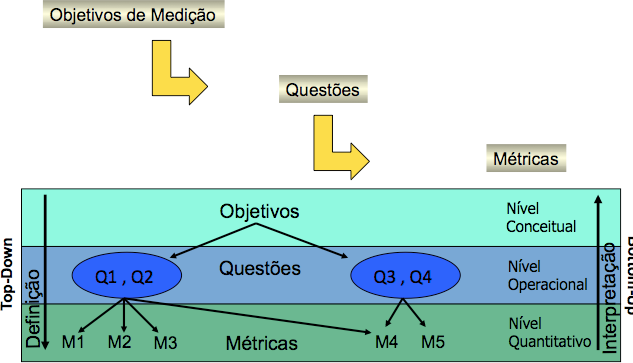
\includegraphics[keepaspectratio=true,scale=0.7]{figuras/GQM_niveis.png}
\caption{Níveis do GQM \cite{sollingen}}
\label{Niveis_GQM}
\end{figure}


A Figura \ref{Niveis_GQM} apresenta três níveis do GQM os quais são detalhados a seguir.

\begin{enumerate}
 \item \textbf{Nível conceitual (Objetivo)}: é um objeto que diz respeito a diversos modelos de qualidade, a partir de vários pontos de vista em um dado ambiente particular. Os objetos de medição podem ser:
 
\begin{itemize}
\item \textbf{Produtos}: são artefatos, resultados e outros documentos que são produzidos durante o processo de desenvolvimento do software. Exemplos: Especificações, casos de teste.

\item \textbf{Processos}: quaisquer atividades se software. Exemplos: Projetar, testar.

\item \textbf{Recursos}: itens que produzem resultados quando usados por processos. Exemplos: Pessoal, hardware.
\end{itemize}

\item \textbf{Nível operacional (Questionamento)}: é um conjunto de perguntas que busca caracterizar se a avaliação/realização de um objetivo específico de acordo com algum modelo característico.

\item \textbf{Nível quantitativo (Métrica)}: é  um conjunto de dados que está associado às perguntas feitas no nível operacional. Pode ser objetiva, ou subjetiva.

\begin{itemize}
\item \textbf{Objetiva}: depende apenas do objeto que está sendo medido e não de opiniões particulares. Exemplo: Tamanho de um software.
\item \textbf{Subjetiva}: não depende apenas do objeto que está sendo medido, mas depende também de um conjunto de opiniões particulares. Exemplo: satisfação do usuário.
\end{itemize}

\end{enumerate}

A estrutura do GQM é mostrada na Figura \ref{Estrutura_GQM}:

\begin{figure}[h]
\centering
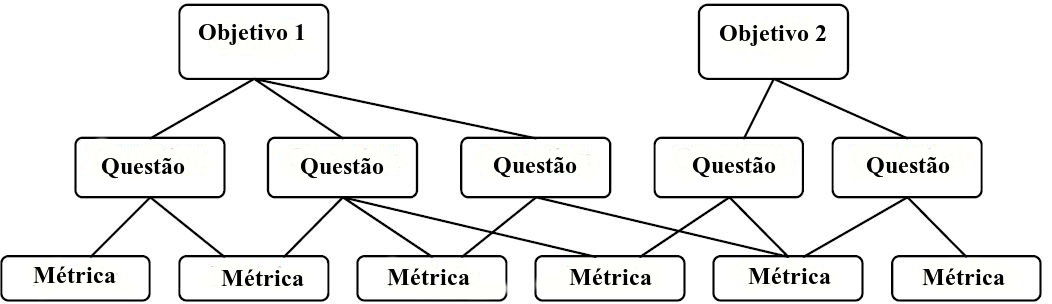
\includegraphics[keepaspectratio=true,scale=0.4]{figuras/GQM_Estrutura.jpg}
\caption{Estrutura do GQM \cite{Basili}}
\label{Estrutura_GQM}
\end{figure}

Com esta estrutura pode-se dizer que a definição das medições se dá a partir de uma abordagem \textit{topdown}, a partir dos objetivos de medição, questões e suas métricas correspondente, enquanto a avaliação ou análise dos resultados se dá por uma abordagem \textit{bottom up}, a partir dos resultados das medições que respondem as questões postuladas e, por sua vez, corroboram os objetivos de medição identificados.

\section{PSM}

O \textit{Pratical Software Measurement} (PSM) é um modelo que estrutura informações com a finalidade de definir medidas que possam ser usadas em um projeto de software \apud{mcgarry}{santos}. Patrocinado pelo departamento de defesa e pelo Exército Norte-Americano, ele tem como objetivo prover um conjunto de práticas, ferramentas e serviços para ajudar os gerentes de projetos a obter informações precisas sobre projetos que estão em andamento, para que estes atinjam suas metas de tempo, custo e qualidade \apud{borges}{deMelo}.	

O PSM foi projetado a partir de três conceitos chaves, são eles \cite{card_jones}:

\begin{itemize}
 \item Necessidade de Informação.
\item Modelo de Informação.
\item Modelo de Processo de Medição.
\end{itemize}

As \textbf{necessidades de informação} são um conjunto de objetivos que servem como insumo para que os gerentes possam monitorar um determinado projeto ou processo de software. As necessidades de informação podem ser obtidas de duas formas \cite{card_jones}:

\begin{enumerate}
 \item Objetivos que o gestor deseja alcançar;
\item Obstáculos que impedem que esses objetivos sejam concretizados. Obstáculos ou questões incluem riscos, problemas e falta de informação em relação a um determinado objetivo.

\end{enumerate}


O PSM organiza-se em sete necessidades de informação \cite{card_jones}, conforme mostra a Tabela \ref{tipos_metricas}.

% \textcolor{red}{Vou explicar em pelo menos uma frase o que é cada necessidade de informação e exemplificar com pelo menos uma métrica.}

\begin{longtable}{|p{100pt}|p{220pt}|p{105pt}|}
 	\caption{Detalhamento das necessidades da informação do PSM.\cite{bailey}} \label{tipos_metricas}\\
 	\hline
 	 {\raggedright \textbf{Necessidade da informação}}
 	 & {\raggedright \textbf{Descrição}}
 	 & {\raggedright \textbf{Exemplo de Medida}}\\
 	\hline
 	 {\raggedright Cronograma e Progresso}
 	 & {\raggedright Relacionados ao  cumprimento de marcos de projeto e à conclusão de unidades de trabalho nos prazos previstos. }
 	 & {\raggedright Datas dos Marcos, Tempo de Folga, Unidades Codificadas.}\\
 	\hline
 	 {\raggedright Recursos e Custo}
 	 & {\raggedright Relacionados à adequação entre o trabalho a ser executado e os recursos alocados ao projeto.}
 	 & {\raggedright Orçamento, custo, Pessoal Alocado, Tempo disponível.}\\
 	\hline
 	 {\raggedright Tamanho e Estabilidade do Produto} 
 	 & {\raggedright Categoriza informações relacionadas à estabilidade das funcionalidades ou à capacidade requerida do software, como também ao volume necessário de software para atender a essa capacidade.}
	  & {\raggedright Linhas de Código, Pontos de Função.}\\
 	\hline
 	 {\raggedright Qualidade do Produto}
 	 & {\raggedright Relacionada à capacidade do software produzido de atender sem falhas às necessidades do usuário.}
 	 & {\raggedright Defeitos, Complexidade Ciclomática, Tempo de Resposta, Conformidade com Padrões, Erros de Operação, Tempo Médio até a Falha.} \\
 	\hline
 	{\raggedright Performance do Processo}
 	 & {\raggedright Relacionada à capacidade do processo de atender às necessidades apresentadas por cada projeto.}
 	 & {\raggedright Produtividade, Defeitos Contidos} \\
 	\hline
 	{\raggedright Eficácia da Tecnologia}
 	 & {\raggedright Trata da viabilidade e adequação das alternativas técnicas propostas, incluindo reuso, maturidade e qualidade dos componentes.}
 	 & {\raggedright Cobertura dos Requisitos.} \\
 	\hline
 	{\raggedright Satisfação do Cliente}
 	 & {\raggedright Relaciona-se ao grau em que os produtos e serviços ofertados atendem às expectativas dos clientes.}
 	 & {\raggedright Grau de Satisfação, Tempo de Suporte.} \\
 	\hline
 	\end{longtable}

 Cada necessidade de informação pode ser decomposta em um conceito mensurável. Um conceito mensurável é uma entidade de uma determinada necessidade de informação \cite{card_jones}.  A Tabela \ref{tipos_metricas3} mostra a necessidade de informação e seus respectivos conceitos mensuráveis.

 \begin{longtable}{|p{185pt}|p{200pt}|}
 	\caption{Conceitos Mensuráveis do PSM.} \label{tipos_metricas3}\\
 	\hline
 	 {\raggedright \textbf{Necessidade da informação}}
 	 & {\raggedright \textbf{Conceito Mensurável}}\\
 	
 	\hline
 	 {\raggedright Cronograma e Progresso}
 	 & {\raggedright 
 	                  Alcance dos Marcos.
 	                  
 	                  Progresso das Unidades de Trabalho.
 	                  
 	                  Capacidade Incremental.
 	                 
	   }\\
 	
 	\hline
 	 {\raggedright Recursos e Custo}
 	 & {\raggedright 
 	                 Esforço do Pessoal.
 	                 
 	                 Desempenho Financeiro.
 	                 
 	              Ambiente e Recursos de suporte.
 	                
 	               } \\
 	
 	\hline
 	 {\raggedright Tamanho e Estabilidade do Produto} 
 	 & {\raggedright  
 	 
	
			 Tamanho e Estabilidade Físicos.
			 
 	                 Tamanho e Estabilidade Funcionais.
		
			
 	                 } \\

 	\hline
 	 {\raggedright Qualidade do Produto}
 	 & {\raggedright
 	                  Correção Funcional.
 	                  
 	                 Suportabilidade - Manutenibilidade.
 	                 
 	                Eficiência.
 	                
 	                Portabilidade.
 	                
 	                  Usabilidade.
 	                  
 	                  Dependabilidade - Confiabilidade.
 	                  
 	             
 	                 
 	          } \\


 	\hline
 	{\raggedright Performance do Processo}
 	 & {\raggedright 
 	                  Conformidade do Processo.
 	                  
 	                 Eficiência do Processo.
 	                 
 	              Eficácia do Processo.
 	                
 	                
}\\
 	
 	\hline
 	{\raggedright Eficácia da Tecnologia}
 	 & {\raggedright 
 	                  Adequação da Tecnologia.
 	                  
 	                  Volatilidade da Tecnologia.
 	              
 }\\
 
 	\hline
 	{\raggedright Satisfação do Cliente}
 	 & {\raggedright 
 	                  Feedback do Cliente.
 	                  
 	                 Suporte ao Cliente.
 	                
}\\
 	
 	\hline
 	\end{longtable}
 
Para \citeonline{mcgarry}, as necessidades de informação são responsáveis por definirem indicadores. Um indicador é constituído por medidas que podem ser uma ou várias medidas básicas que por sua vez servem para construir medidas derivadas. Indicadores, medidas derivadas, medidas base e entidades são usados para construir medições como mostra a Figura \ref{PSM}: 

\begin{figure}[h]
\centering
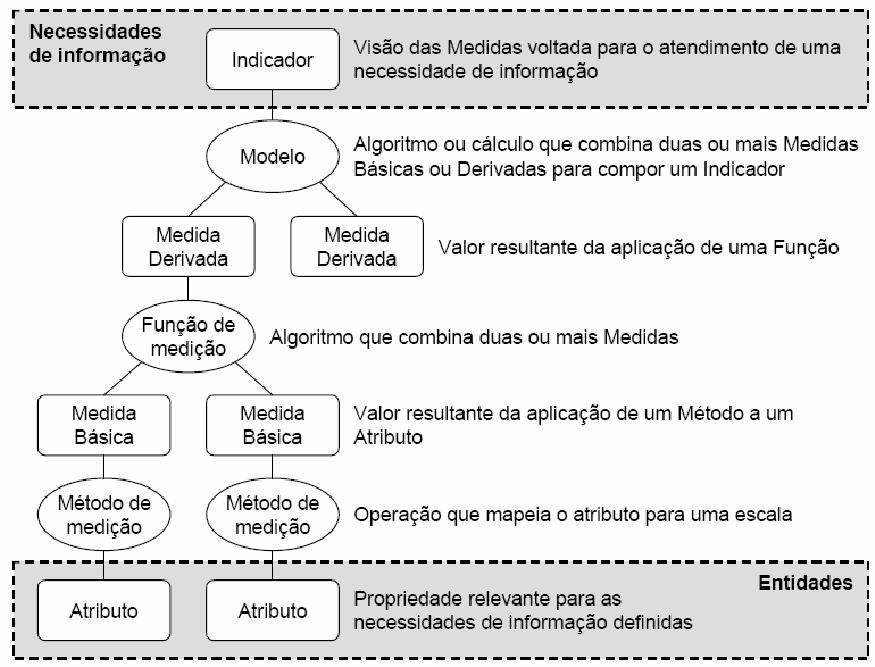
\includegraphics[keepaspectratio=true,scale=0.4]{figuras/PSM.jpg}
\caption{Construtor de Métricas \cite{mcgarry},\cite{borges} }
\label{PSM}
\end{figure}

O \textbf{modelo de informação} define uma relação entre as necessidades de informação mapeadas pelo gestor e os dados dos objetivos que serão coletados (medidas). O modelo de informação também fornece ideias básicas para a medição. Este modelo é definido em três níveis:

\begin{enumerate}
\item Medidas básicas
\item Medidas derivadas
\item Indicadores
\end{enumerate}

A organização do modelo de informação do PSM é mostrada na Figura \ref{Modelo_PSM}.

\begin{figure}[h]
\centering
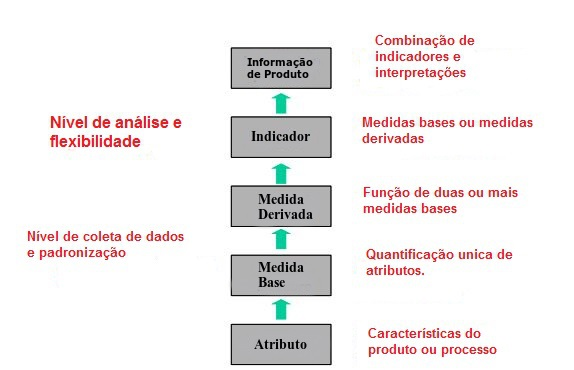
\includegraphics[keepaspectratio=true,scale=0.8]{figuras/Modelo_Psm.jpg}
\caption{Modelo de Informação do PSM \cite{card_jones} }
\label{Modelo_PSM}
\end{figure}

Da perspectiva do \textbf{modelo de processo de medição}, o PSM define quatro atividades básicas, são elas \cite{card}:

\begin{itemize}
\item Planejar Medição: Essa atividade consiste em compreender as necessidades da informação do projeto e a definição de métricas que sejam adequadas para atender essas necessidades.
\item Executar Medição: Essa atividade consiste na execução do modelo de informação definido na fase anterior, para que se possa chegar aos resultados esperados e que assim possa servir de insumo para que a melhor decisão possa ser tomada pela equipe de Software.
\item Avaliar Medição: Essa atividade tem como objetivo investigar se o processo está dentro do aceitável. Para que isso seja possível é avaliar o processo de medição e avaliar informações do produto.
\item Consolidar Medição:  Essa atividade tem como objetivo obter o comprometimento da empresa em relação as medições definidas.

\end{itemize}

Desta forma o PSM é um guia bastante recomendado para empresas que desejam implantar a qualidade de software e ao mesmo tempo manter a gerência dos seus produtos.


%\textcolor{red}{colocar a justificativa do porque do uso do GQM aqui motivando o proximo capítulo de aplicação.}

Para o presente trabalho será usada uma abordagem GQM para a definição de métricas. A abordagem será  \textit{top-down}, e terá como objetivo determinar um conjunto de metas e medidas para gerar métricas que servirão de apoio para a seleção de produtos CMS. O GQM foi escolhido, porque é necessário neste trabalho uma profundidade grande a respeito do levantamento de métricas.


